%!TEX encoding = UTF-8 Unicode
%!TEX root = ../lect-w08.tex

% \Subsection{TODO TABORT Integrerad utvecklingsmiljö (IDE)}

% \begin{Slide}{\TODO TABORT Välja IDE}\SlideFontSmall
% \begin{itemize}
% \item En \Emph{integrerad utvecklingsmiljö} \Eng{Integrated Development Environment, IDE} innehåller \\ editor + kompilator + debugger + en massa annat\\och gör utvecklingen enklare när man lärt sig alla finesser.

% \item Läs om vad en IDE kan göra i appendix.

% \pause

% \item På LTH:s datorer finns tre populära IDE installerade:
% \begin{enumerate}\SlideFontSmall

% \item \Emph{VS Code} med tillägget Metals. \Alert{Rekommenderas!}
% \begin{REPL}[numbers=none]
% > code
% \end{REPL}


% \item \Emph{IntelliJ IDEA} med Scala-plugin. Välj denna om du vill ha en IDE som är mer avancerad och är sugen på att lära dig något nytt.
% \begin{REPL}[numbers=none]
% > idea
% \end{REPL}

% \item \Emph{Eclipse} med plugin \Emph{ScalaIDE} förinstallerad, men rekommenderas ej då den ligger efter i Scala-version.
% \begin{REPL}[numbers=none]
% > scalaide
% \end{REPL}

% \end{enumerate}
% %Läs mer om dessa i appendix.
% %  innan du väljer vilken du vill lära dig.
% % \\Där står även hur du installerar dem på din egen dator.
% % \\IntelliJ anses av många för tillfället ha det bästa Scala-stödet, men är du van vid Eclipse så kanske du vill använda ScalaIDE.
% \end{itemize}
% \end{Slide}

% \begin{Slide}{\TODO SKA HANDLA OM DEBUG i VS Code med Scala-plugin Metals}
% 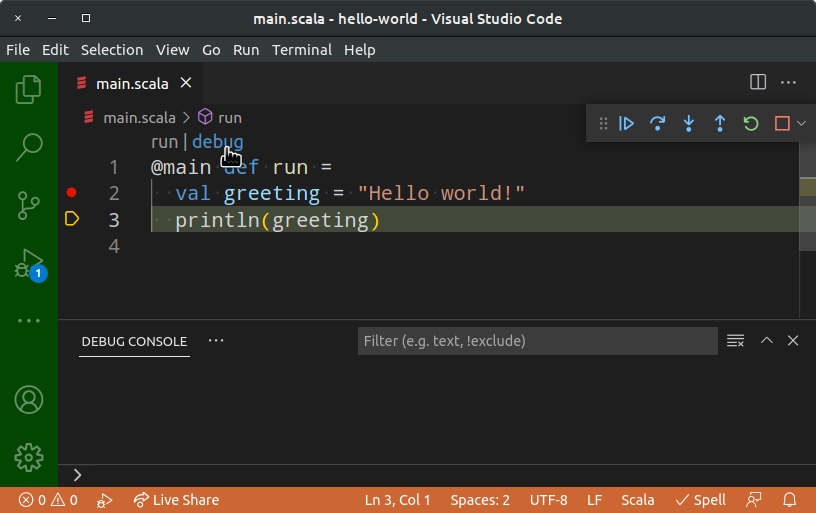
\includegraphics[width=\textwidth]{../img/vscode-debug.png}
% \end{Slide}
  

% \begin{Slide}{IntelliJ IDEA med Scala-plugin}
% 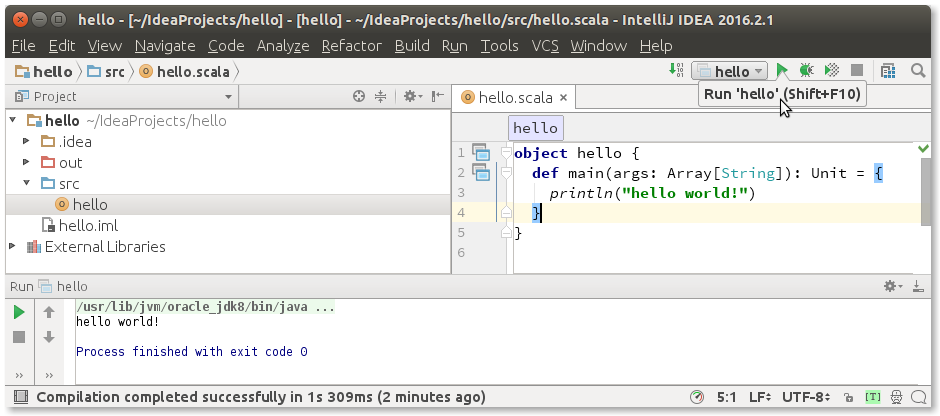
\includegraphics[width=\textwidth]{../img/intellij/idea-hello.png}
% \end{Slide}

% \begin{Slide}{Eclipse med ScalaIDE}
% 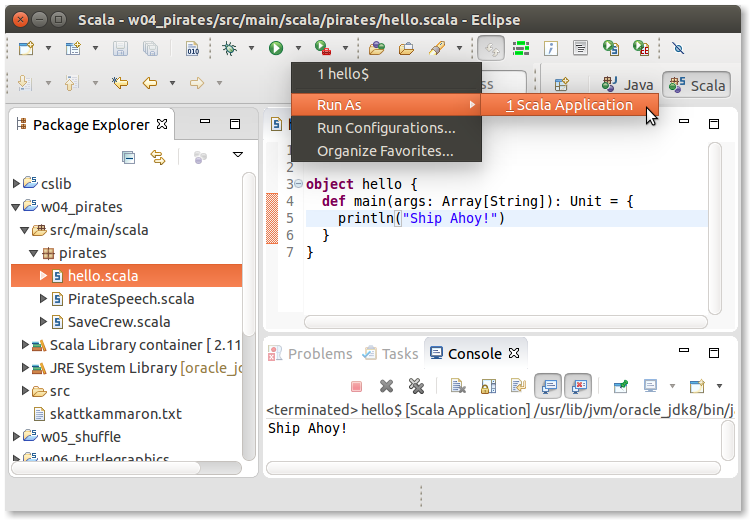
\includegraphics[width=\textwidth]{../img/eclipse/eclipse-pirates-hello.png}
% \end{Slide}

